\documentclass[msc]{ppgccufmg}

\usepackage[english]{babel}
\usepackage[T1]{fontenc}
\usepackage[utf8]{inputenc}

\usepackage[
    english,
    bookmarks=true,
    bookmarksnumbered=true,
    linktocpage,
    colorlinks,
    citecolor=black,
    urlcolor=black,
    linkcolor=black,
    filecolor=black
]{hyperref}
\usepackage[square]{natbib}

\begin{document}

\ppgccufmg{
    title={Improving D2D Multi-Hop Message Forwarding},
    portuguesetitle={Melhorando o Encaminhamento de Mensagens em Redes D2D com Múltiplos Saltos},
    authorrev={da Silva, Michael Dougras},
    university={Federal University of Minas Gerais},
    portugueseuniversity={Universidade Federal de Minas Gerais},
    course={Computer Science},
    portuguesecourse={Ciência da Computação},
    address={Belo Horizonte - Minas Gerais},
    date={2018-06},
    keywords={d2d, multi-hop, network, forwarding},
    advisor={Antônio Alfredo Ferreira Loureiro},
    abstract={Abstract}{abstract},
    dedication={dedication},
    ack={acknowledgement},
    epigraphtext={Not everything that counts can be counted, and not everything that can be counted counts.}{William Bruce Cameron - "Informal Sociology: A Casual Introduction to Sociological Thinking"}
}

\chapter{Introduction}
\label{ch:Introduction}

Mobile devices have become smaller and more powerful over the years. Smartphone based computing and communication has become ubiquitous.
Connected services and applications like social networks, instant messaging apps, content distribution systems and games, for example, have imposed several traffic growth in the mobile network.
To support this demand we have been improving the network infrastructure. In indoor environments this strategy is feasible, because usually
they are smaller and we have more control over the number of devices. However when we are dealing with outdoor environments this approach can be
unfeasible, because in this case we have a dynamic scenario in which the number of devices and consequently the traffic demand can be unpredictable.

In the current mobile communication model devices must contact a base station to communicate with other devices or services.
Recent works have explored a new communication model in which mobile devices can bypass the base station to communicate directly
with near devices. This model is called Device to Device communication or D2D \cite{yang2013solving}. This approach has several applications,
for example offload traffic from base stations~\cite{yang2013solving,nunes2016leveraging,aijaz2013survey,pyattaev2013proximity,andreev2014cellular,bastug2014living},
to provide proximity based services \cite{lin2014overview} and  to provide extended network coverage under emergency scenarios \cite{babun2015multi}.

The D2D communication shows itself as a sensible solution to evolve the mobile network system and improve the devices experience. However there
are some characteristics of this scenario that makes the regular Internet communication protocols unapplicable. One of the major characteristics is
the absence of end-to-end path between two nodes. This occurs because messages are transmitted when there are contacts between two or more nodes, and
these contacts are defined by people mobility. This fact by itself makes the IP protocol routing mechanism unapplicable, which makes the routing problem
one of the major topics of study \cite{misra2016opportunistic}. Other characteristic is the intermittently connections also caused by nodes mobility. In the regular IP protocol nodes
after receiving a packet immediately forwards it to the next hop based on its routing table. Due to intermittently connections, nodes can't forward the message
immediately in some cases.

These problems were discussed and solutions were proposed in the context of Disruption Tolerant Networks (DTNs) \cite{fall2003delay}.
Regular networks are based on the \textit{store-and-forward} paradigm, in which nodes after receiving a message
immediately forward it to other connected node that can help to deliver the message to the destiny. DTN networks define the \textit{store-carry-and-forward} paradigm,
in which a node after receiving a message, it stores it in a persistent buffer, and carries it until there is a proper contact to forward the message.

The \textit{store-carry-and-forward} paradigm solves the primary problem of communication, making it possible to transmit a message from a node to another, however there is still some problems to solve.
One of the major problems is the connection establishment. In D2D networks the communication process is highly dependent of nodes cooperation and resource sharing. Regarding the connection establishment
there is a discussion of the best interface to use. Some works propose the spectrum sharing between D2D connections and regular mobile network connections \cite{lin2014spectrum}. The major benefit of using this
approach is the higher network performance and the major challenge is to define a good spectrum allocation mechanism to evict communication interference between closer devices and base stations.
Some works propose the use of secondary interfaces like WIFI and bluetooth \cite{mao2015contact}. The major benefit of this approach is the reduced interference with closer connections and
simplified connection establishment mechanism. The major problem is the reduced network performance.

With a defined communication interface and the data transmission paradigm \textit{store-carry-and-forward} it is possible to forward messages in the network using only D2D communications.
However there still an interesting problem to solve: the routing protocol. As said earlier in this scenario there is no predefined end-to-end path between two nodes, so the regular IP routing mechanism does not work \cite{misra2016opportunistic}.
There are several proposals to solve this problem, in which the major solutions are based on flooding variations, probability functions and social context exploration.
We will discuss the major solutions in depth in the next chapter. One thing to notice is that the algorithms based on utility functions (probability and social context based strategies, mainly)
tend to concentrate the network traffic in some nodes with higher utility values, penalizing them \cite{chilipirea2013energy}. This is a remarkable problem, because
in networks that use the \textit{store-carry-and-forward} paradigm nodes need to allocate a buffer to store messages until there is chance to forward it. If the traffic is too high, some nodes can have problems of
buffer overflow \cite{silva2015survey}.

This work has two major contributions. First we propose a new buffer management strategy called \textit{Space Time Drop} or just ST-Drop that aims to solve the problem of buffer management under high traffic demands.
The proposed solution shows a notable performance when combined with social aware and probability based routing algorithms, outperforming classic approaches.
The second contribution is the definition of a distributed implementation of a new social aware routing algorithm called Groups-NET proposed in \cite{nunes2016leveraging}.
We propose a distributed algorithm for detecting and manage groups. The initial experiments show that the algorithm outperforms the BubbleRap algorithm on network overhead metric with compatible delivery ratio.
The work is organized as follows. In chapter \ref{ch:MessageForwarding} we discuss the main approaches and algorithms to forward messages in D2D networks. This chapter introduce important
concepts to understand the proposed solutions. In chapter \ref{ch:StDrop} we discuss the classic approaches of buffer management and introduce the proposed algorithm ST-Drop.
In chapter \ref{ch:GroupsNet} we introduce the distributed implementation of the Groups-NET algorithm and present some initial results. And in chapter \ref{ch:Conclusion} we conclude the work
with a summary of the main results and discuss future works to expand the research.
\chapter{Groups NET Distributed Implementation}
\label{ch:GroupsNet}

In D2D networks communication is established when a contact occurs, and the contacts are driven by human mobility.
Therefore understanding human mobility and how people interact is a fundamental requirement to create good solutions in this scenario.
Recent works have shown that the best solutions for D2D communication are those based on social context, mainly those that explore how
people interact in groups or communities. In this chapter we propose a distributed implementation of Groups-NET, a forwarding algorithm
based on group encounters \cite{nunes2016leveraging}. We propose an algorithm for group detection and tracking in a distributed environment
and used this to implement Groups-NET. Through experiments with a real mobility trace containing 115 nodes we show that the solution achieves
a good delivery ratio with an expressive lower network overhead when compared with the state-of-art BubbleRap algorithm.

<Write down the chapter structure when finished>
% This chapter is organized as follows. The section \ref{sec:groupsNet} details the original Groups NET implementation as is proposed in \cite{nunes2016leveraging}.
% The section \ref{sec:distributedGroupsNET} details the proposed distributed implementation inspired by the original Groups NET. This sectio is divided in two parts: in
% \ref{subsec:subsec:groupDetection} the grouping detection algorithm is detailed and in \ref{subsec:forwardingDistGroupsNET} the forwarding decision is also detailed.
% In section \ref{sec:GNExperiments}

\section{The Groups NET Algorithm}
\label{sec:groupsNet}

Groups-NET is a multi hop and multi copy forwarding algorithm for D2D networks that explores people group meetings to propagate content.
A group is defined as a set of people that are together in a place due to a common goal. For example, people working in the same company or students attending the same class.
The algorithm is based on the idea that group encounters show some regularity along the time, because in general people have regular schedules and routines. Therefore we
can explore group encounters to forward messages. In their previous work, \citet{groupMobility} proposed an algorithm for group detection and tracking, in which
detected groups show encounters regularity along the time, mainly on daily and weekly basis. This algorithm operates on contact traces.

First, the contact trace is split considering time windows of a predefined size. Contacts in each time window are used
to create contact graphs, in which vertices denotes devices and edges denotes contacts in that time window. After this
a sequence of graph contacts along the time is created, representing people contacts along the time. For each of these graphs
the clustering algorithm Clique Percolation \cite{derenyi2005clique} is executed, to find clusters based on the contacts of a time interval.
A cluster in a contact graph represents a group encounter in a that time interval. In order to find groups that have encounters in different time windows
the authors introduced the \textit{Group Correlation Coefficient} metric, which measures the similarity of two group captured in distinct contact graphs returning a value
between 0 and 1. It is defined as the number of intersection members of the two groups divided by the number of members of the union of the groups.

<Finish to explain how the forwarding decision is defined based on group encounters>

<Discuss the centralized nature of this solution and talk about the major challenges to develop>

<The following sections were not revised yet, I put just some notes to guide me>

\section{Distributed Groups NET}
\label{sec:distributedGroupsNET}

In this section we propose a distributed implementation of Groups NET forwarding algorithm. The solution is
comprised of two stages: The first stage is group detection, in which nodes use neighborhood discovery to
infer social group meeting using a local algorithm. The second stage is message forwarding, in which nodes
use the generated group data to decide when to forward a message or not. The following sections describe in
details the two stages.

\subsection{Grouping Detection and Tracking}
\label{subsec:groupDetection}

The mobile group detection algorithm proposed here is derived from the ideas presented in \cite{groupMobility}.
A group is defined as a set of people that get in contact on a given point of space and time. The authors show that
group encounters have some level of regularity along the time (mainly at daily and weekly basis). This property can be used by forwarding algorithms.

In the original proposal the authors use a approach to detect groups based on global network knowledge. They basically
build a contact graph considering a predefined time interval, and for each graph is used the Clique Percolation community
detection algorithm. Each community detected by the algorithm is considered a group meeting in that time window. Then
a metric called \textit{Group Correlation Coefficient} is used to detect instances of the same group across multiple time
windows.

With this approach the authors show that groups usually have regular encounters along the time (specially in daily and weekly basis).
But they also discuss that the detection approach is unfeasible for a distributed environment, because it assumes a global network
knowledge. However, authors also discuss that implementing a distributed solution for this should be a simple task, because in the local
scope nodes can use neighborhood discover strategies and process regular neighbors encounters to decide their group encounters.

In this work we expanded this idea to build a distributed solution for group detection.It is composed of four processes
that are executed concurrently by each node using basically neighborhood inspection and some basic additional parameters. In the following sections each process is explained.

\subsubsection{Device's Local Group Detection}

This process is responsible for processing nodes' local contacts and decide when a group meeting happens.
The algorithm is very simple. Each node keeps two lists of devices. The first is the \textit{friends} list (lets call it FL)
that keeps track of current nodes considered as friends, i.e, members of a group that have a recent encounter.
The second list is the \textit{strangers} list (lets call it SL), that keeps track of recent nodes' contacts that are not yet
considered as friends. Each entry in these lists have a contact counter that keeps track of consecutive
contacts with that node, and also have a inactive counter that keeps track of consecutive periods of time
without contact with that node.

The node inspects its neighborhood at each predefined \textit{time interval} and based on current neighbors
it updates the friends and strangers list. This update is based on two predefined parameters: the \textit{friend threshold}
and \textit{inactive threshold}. Lets call these parameters as FT and IT respectively. Based on these parameters the following
steps are executed:

\begin{itemize}
	\item At each time interval a node collects its current neighbors (lets call it CN).
	\item The first step is to update the counters of friends list. For each current neighbor that is present in the friends
	list, we increase the contact counter and reset the inactive counter. For each node present in the friends list that is
	not a current neighbor we reset the contact counter and increase the inactive counter.
	\item The second step is to update the strangers list. For each current neighbor that is present in the strangers list
	we reset the inactive counter and increase the contact counter. If the contact counter reaches the friend threshold
	the node is promoted to friends list. For each node that is present in strangers list but is not a current neighbor
	we reset the contact counter and increase the inactive counter. If the inactive counter reaches the inactive threshold
	the node is removed from the strangers list. Nodes that are current neighbors and are not present in both friends and strangers
	list are added in the strangers list with contact counter equals 1.
	\item As a final step, we check the number of nodes in the friends list that are considered inactive. A node is considered
	inactive when the inactive counter reaches the inactive threshold. If more than 50 percent of the nodes in the friends list
	is inactive, the friend list is archived and considered as a group meeting that happened in the past. When this happens we
	clear the friends and strangers list and restart the algorithm.
\end{itemize}

In the end this algorithm creates a list of local detected group meetings. This list is used by the local group combination process to
detect instances of the same group with multiple encounters along the time.

\subsubsection{Local Group Combination}

In this step each mobile device process groups discovered in the previous step to discover groups that
have multiple encounters along the time. The algorithm is based on a metric called \textit{Group Correlation Coefficient} defined in [add-reference]. This metric basically computes the proportion of nodes shared between two sets.

Each node keeps a list of \textit{combined groups}, that keeps track of groups with multiple encounters along the time. For each
local group detected in the previous process, we check if there is a combined group with Group Correlation Coefficient greater or equals 0.5.
If there is, the local group is combined into the combined group adding its members to it and registering a new encounter. If there isn't, a new combined group is initialized with the local group data.

The combined groups generated in this process are used by neighborhood inspection to compose the final groups considered in the forwarding algorithm.

\subsection{Neighborhood Inspection}

Besides inspecting its current neighborhood, at each considered time interval each node also collects its neighbors combined groups. The collected groups are combined with the groups generated by the local group combination process using the same approach described previously. Groups that have correlation coefficient greater of equals 0.5 are merged. This step is used to expand a node local vision with its neighbor
network knowledge. So, in the end the local combined groups are updated with neighbors detected group information.

\subsubsection{Group Graph Creation}

In this step we build the graph of groups using the combined groups created by the neighborhood inspection process. The graph is created using the approach described in \cite{groupMobility}

\subsection{Forwaring Decision}
\label{subsec:forwardingDistGroupsNET}

\section{Experiments}
\label{sec:GNExperiments}

\section{Results}
\label{sec:GNResults}

\section{Conclusion}
\label{sec:GNConclusion}


\section{The Distributed Groups NET}



\subsection{Mobile Group Detection}




\chapter{ST-Drop: A Novel Buffer Management Strategy}
\label{ch:StDrop}

In D2D multi-hop forwarding protocols nodes need to cooperate and act as relays to messages of other nodes. As a result of this cooperative behavior,
each node needs to share its resources with the network allocating memory to the message in a buffer. This buffer is used to store messages being forwarded temporarily, and its capacity is limited. Consequently, the network traffic load, combined with the way a given forwarding algorithm operates, can overflow the devices’ buffers. In single-copy protocols this problem is alleviated because the number of messages in the network is relatively lower. However, in multi-hop protocols this is a real problem because multiple copies of a message are spread in the network, so the traffic can grow very quickly. Besides allowing multiple copies of a message, a central entity with global network knowledge usually does not exist. As a consequence, nodes do not know when a message is delivered to the destination. Even when the message is delivered in multi copy forwarding algorithms, copies of this message remain in the network until they exceed their TTLs (time to live) or are dropped by other mechanism \citep{bindra2012need}. Therefore, a good buffer management mechanism is a critical requirement in this scenario.

This chapter presents a buffer management algorithm for D2D multi-hop and multi copy forwarding algorithms, named Space-Time Drop (ST-Drop). This algorithm explores the local information to measure the time and space coverage of the message in the network. The basic idea is that a message with higher time and space coverage is more likely to have
been delivered, so it can be dropped first. Through experiments with a real mobility trace containing 115 nodes and a synthetic mobility trace containing 500 nodes, we show that ST-Drop enables routing protocols to achieve a good delivery ratio with low network overhead. With the purpose of evaluating the performance of ST-Drop when applied to different types of opportunistic routing algorithms, we consider an epidemic based, a probabilistic, and a social-aware algorithm. Using three well-known forwarding algorithms, we show that ST-Drop helps the forwarding protocols to achieve a good delivery ratio with low overhead.

\section{Buffer Management in D2D Networks}

In D2D networks, users must devote a fraction of their devices’ storage to be used as a buffer that temporarily stores the messages carried by them.
The basic idea to manage such buffer, to avoid its overflow while maintaining opportunistic forwarding efficiency, is to use congestion control mechanisms. \citet{silva2015survey} have classified congestion control mechanisms and provided an extensive review of message drop policies used in opportunistic networks. In this section, we go over some of the state-of-art message drop policies highlighting their specific features.

\citet{lindgren2006evaluation} proposed the Evict Most Forwarded (MOFO) drop policy, which uses the idea that a message forwarded a large number
of times has a higher probability to be delivered, even if it is dropped locally. They also proposed the Evict Shortest Life Time First (SHLI) drop policy, which is based on the idea that it makes more sense to spend resources on messages that have higher TTL, because, intuitively, these messages have a higher probability to be delivered. The Drop Largest policy \citep{rashid2010efficient} selects big size messages to drop first, because, by doing this, more space is freed from the buffer. Another basic policy is FIFO, in which, as the name suggests, messages that arrived first are dropped first.

\citet{rashid2013message} proposed the Message Drop Control Source Relay (MDC-SR) buffer management algorithm, in which nodes stop receiving incoming messages when the buffer occupancy achieves a defined upper bound, except when the node is the destination of the message. With this approach, the algorithm decreases the number of message drops in the network. Through experiments, they showed that MDC-SR optimized the performance of Epidemic, Prophet and First Contact routing algorithms regarding delivery ratio and
network overhead.

\citet{krifa2008optimal} proposed the Global Knowledge Based Drop (GBD-Drop) buffer management algorithm, in which they first assume a global knowledge of the network to decide which messages to drop, achieving optimal performance. They proposed a distributed version of the algorithm that uses statistic learning to approximate the global knowledge
of the network. Through experiments, they showed that the centralized and distributed versions of the algorithm outperform the basic drop policies. The GDB-Drop can also be configured to achieve a better average delivery delay or better average delivery ratio.

\citet{rashid2011drop} proposed the E-Drop buffer management algorithm, in which messages with size greater or equal to the incoming message are dropped first. In the case of an incoming message with a size greater than the messages in the buffer, it works like the FIFO policy. This policy minimizes the drop of messages because it will usually remove only one message from the buffer to receive the incoming message. Through simulations, using mobility models, they show that E-Drop
outperforms the MOFO algorithm.

\citet{li2009n} proposed the N-Drop buffer management algorithm, in which messages transmitted more than a predefined constant are dropped first. Through simulations, they showed that this algorithm outperforms FIFO when used with Epidemic routing algorithm. \citet{ayub2010t} also proposed the T-Drop buffer management algorithm, in which
messages with size in a predefined range $T$ are dropped first. Through simulations, the authors show that this algorithm outperforms FIFO when applied to the routing algorithms Epidemic and Prophet.

\citet{naves2012lps} proposed two new buffer management policies. The first one is named Least Recently Forwarded (LRF), and it drops messages that were forwarded more recently. The second one is named Less Probable Sprayed (LPS), and it drops messages that have less probability to be delivered first. Through experiments with Epidemic and Prophet
routing algorithms using real-data traces, the authors showed that both algorithms outperform FIFO and MOFO in delivery ratio and overhead.

The aforementioned buffer management algorithms are based on only one local metric, for example, buffer time, forward count, TTL, and message size. These metrics represent a good choice because they are independent of the routing algorithm. However, their isolated meaning can be insufficient to decide whether to drop a message or not. We have combined basic metrics to create a new buffer management algorithm named Space-Time Drop (ST-Drop). In the following section, we describe the ST-Drop algorithm.

\section{The ST-Drop Algorithm}
\label{sce:stDrop}

The ST-Drop formulation starts with the idea that a message with a greater space and time coverage in the network has a greater probability to have been already delivered, so it can be dropped first. Based on this idea, we have defined a space coefficient $S_{c}$ that measures the space coverage of the message in the network, and the time coefficient $T_{c}$ that measures the time coverage of the message in the network. Therefore, to compute the space-time coverage $ST_{c}$, we use the simple function:

\begin{equation}
    ST_{c} = S_{c} \cdot T_{c}.
\end{equation}

With this first formulation, we do not define how to compute $S_c$ and $T_c$. Buffer management algorithms for D2D networks are ideally implemented in a distributed way, so we have to be restricted to local information. Besides this, we want to keep ST-Drop independent of the routing algorithm. Consequently, we decided to combine the metrics used by the basic algorithms to compute our defined metrics $S_c$ and $T_c$.

The first issue is how to measure space coverage. In cellular networks, the contacts are driven by human mobility. Intuitively we can say that a message carried by only one person will have fewer opportunities to be forwarded than a message carried by two or more people because it will be restricted to the mobility of only one person. Thus, we can say that the
number of devices carrying a message is a sensible measure of the space coverage of the message, because the space coverage of a message is a direct result of the combination of the devices' mobility. Therefore, we use the same metric used by the MOFO algorithm to measure the space coverage, i.e., the number of times a message was forwarded by a node.
The forward counter is a local measure of the number of devices carrying a message.

The second issue is how to measure the time coverage. FIFO exploits the time the messages have been carried by a node to decide which message to drop first. Using only this metric we could drop a recently created message and let a message with almost ending TTL in the buffer. SHLI uses the TTL of messages to decide which message should be dropped first. Using only this metric we could let a message with a huge TTL indefinitely in the buffer of a node that has a low delivery probability for it. Also, in a real scenario, messages may have different TTL values. Thus, messages with relatively low initial TTL would be penalized. Therefore,
ST-Drop combines the idea of FIFO and SHLI, normalizing the carrying time $CT$, that is the time a message is stored in the buffer of a node, with the TTL of the message, defining $T_{c}$ as:

\begin{equation}
    T_{c} = \frac{CT}{TTL}.
\end{equation}

With this formulation, we can now compute the space-time coverage using only local information. The ST-Drop policy is formalized in Algorithm \ref{alg:stDrop}. ST-Drop is called only when there is no available space in the buffer to receive an incoming message. The algorithm sorts the messages in reverse order by their $ST_c$ values and stores them in a list. The messages with $ST_c$ equals 0 are removed from the list, which implies that they will never be dropped. The algorithm considers that
dropping a message with space-time equals 0 is not fair, because the message was not forwarded so far. Then, the first message of the list is dropped until enough space is freed for the new message or the list becomes empty. If enough space is freed, then the algorithm returns a confirmation to receive the incoming message. Otherwise, the device must reject the incoming message.

\begin{algorithm}

 \caption{ST-Drop algorithm}
 \label{alg:stDrop}
 \begin{algorithmic}[1]
 \renewcommand{\algorithmicrequire}{\textbf{Input:}}
 \renewcommand{\algorithmicensure}{\textbf{Output:}}
 \REQUIRE incomingMessage
 \REQUIRE buffer
 \ENSURE  receive
 %\\ \textit{Check if the incoming message size is higher than the buffer capacity}
  \IF {incomingMessage.size > buffer.capacity}
    \RETURN false
  \ENDIF
 \\ \textit{Sort the messages in reverse order by $ST_c$} :
  \STATE msglist = sort(buffer)
 \\ \textit{Remove messages with $ST_c = 0$}
  \STATE msglist.filter()
 \\ \textit{Drop messages until enough space is freed}
  \STATE incsize $\leftarrow$ incomingMessage.size
  \STATE available $\leftarrow$ buffer.availablespace
  \WHILE {available < incsize and not msgList.empty}
    \STATE msg $\leftarrow$ msglist.removefirst()
    \STATE buffer.drop(msg)
    \STATE available $\leftarrow$ available + msg.size
  \ENDWHILE
  \IF {available < incsize}
  \RETURN false
  \ELSE
  \RETURN true
  \ENDIF
 \end{algorithmic}
 \end{algorithm}

\section{Simulation Methodology}
\label{sec:experiments}

In this section, we describe the simulations we have performed to evaluate ST-Drop. Firstly, we describe the metrics for D2D opportunistic communication that we have evaluated, and then we present the opportunistic routing algorithms in which we have applied ST-Drop. Next, we describe the two mobility traces used to emulate the network nodes' mobility and
their proximity contacts, and finally we discuss the parameters and configurations we used in our experiments.

\subsection{Metrics}

With the goal of comparatively evaluating ST-Drop with other message drop policies, we used the following traditional opportunistic network metrics:

\begin{itemize}
\item \textbf{Delivery ratio:} evaluates the percentage of successfully delivered messages along the time;
\item \textbf{Network Overhead:} measures the number of retransmissions per created message in the network, i.e., the number of D2D transmissions that each algorithm performs along the time normalized by the number of created messages.
\end{itemize}

Message drop policies for D2D networks should achieve cost-effective delivery considering these metrics, i.e., the highest possible delivery ratio with the lowest possible network
overhead. Successfully delivered messages are those which the base station will not need to deliver itself, thus using less bandwidth. A high number of message re-transmissions (high overhead)
may negatively impact the users' experience by, for example, increasing devices' energy expenditure.

\subsection{Opportunistic Forwarding Algorithms}
\label{sec:routingAlgorithms}

We used algorithms based on three different approaches to study the behavior of our solution when integrated with different routing algorithms.
The first routing algorithm is the Epidemic \citep{vahdat2000epidemic}, also known as Flooding. This algorithm is considered one of the most basic ones
as it is not based on utility functions or similar metrics. In this algorithm, at each encounter between two nodes, they exchange all the messages they have in their respective buffers. The second routing algorithm that we considered is the Prophet \citep{lindgren2003probabilistic}. This algorithm uses a delivery probability as a utility function to decide whether to
forward a message or not. And the third is the Bubble Rap \citep{hui2011bubble}. It is a social-aware algorithm based on the concept of community and network node's popularity. These algorithms are presented with more details in chapter \ref{ch:MessageForwarding}.

We are using routing algorithms based on epidemic routing, probabilistic functions, and social-aware strategies. In this way, we can evaluate the impact of different types of routing algorithms when using ST-Drop.

\subsection{Mobility Traces}
\label{sec:datasets}

We have used two mobility traces to emulate nodes' mobility. The first one is the NCCU trace \citep{tsai2015nccu}, a real-world dataset that monitors the mobility of 115 students inside a campus for 15 days. The second one is a synthetic trace generated by the Small World in Motion (SWIM) mobility model \citep{swim-secon10}. This trace is based on a state-of-the-art mobility model that captures the existence of social communities influencing human mobility, and it simulates the mobility of 500 people for 11 days. We have chosen the two traces to test ST-Drop
under different network scales.

\subsection{Execution}
\label{sec:simulation}

We used The ONE simulator \citep{keranen2009one} to emulate the execution of the opportunistic routing algorithms using different message dropping policies. It is a discrete event simulator focused on opportunistic networks. By default, the simulator does not support custom buffer management algorithms and the Bubble Rap routing algorithm, therefore we implemented these features\footnote{The source code is available at https://github.com/micdoug/the-one/tree/58e207ac44d5012fac5d103da781d30266164216}.

To test the ST-Drop, we defined the buffer capacity and a network traffic model. As discussed in \citep{grasic2012analysis}, there is no pattern when it comes to defining a traffic model to test solutions in this scenario. Thus, we chose sensible values in our simulation. The buffer capacity was defined as 1GB. Messages have seven days of TTL and are generated
at random times within the trace duration. Message sizes are chosen from the interval [50MB,100MB] with uniform probability. The source and destination pair for each created message is also selected with uniform probability among the nodes in the network.

We have defined two network traffic load levels based on the number of nodes of each scenario. The first load level generates messages equals to 50\% of the number of nodes at each day, and the second generates 100\%. Table \ref{tab:trafficLevels} summarizes the number of messages generated in each traffic load level:

\begin{table}[H]
\centering
\caption{Network Traffic Load Scenarios}
\label{tab:trafficLevels}
\begin{tabular}{|c|c|c|c|}
\hline
\multicolumn{2}{|c|}{\textbf{Scenario}} & \textbf{Messages/Day} & \textbf{Total} \\ \hline
\multirow{3}{*}{NCCU}       & 50        & 58                    & 522            \\ \cline{2-4}
                            %& 75        & 86                    & 774            \\ \cline{2-4}
                            & 100       & 115                   & 1035           \\ \hline
\multirow{3}{*}{SWIM}       & 50        & 250                   & 1250           \\ \cline{2-4}
                            %& 75        & 375                   & 1875           \\ \cline{2-4}
                            & 100       & 500                   & 2500           \\ \hline
\end{tabular}
\end{table}

We have emulated each scenario with each traffic level 10 times using different seeds to generate message's sources and destinations, and messages size.
The average delivery ratio and the average network overhead of each scenario were computed and presented with 95\% confidence intervals.

\section{Results}
\label{sec:results}

% images nccu 100
\begin{figure}
    \begin{subfigure}[b]{0.5\columnwidth}
        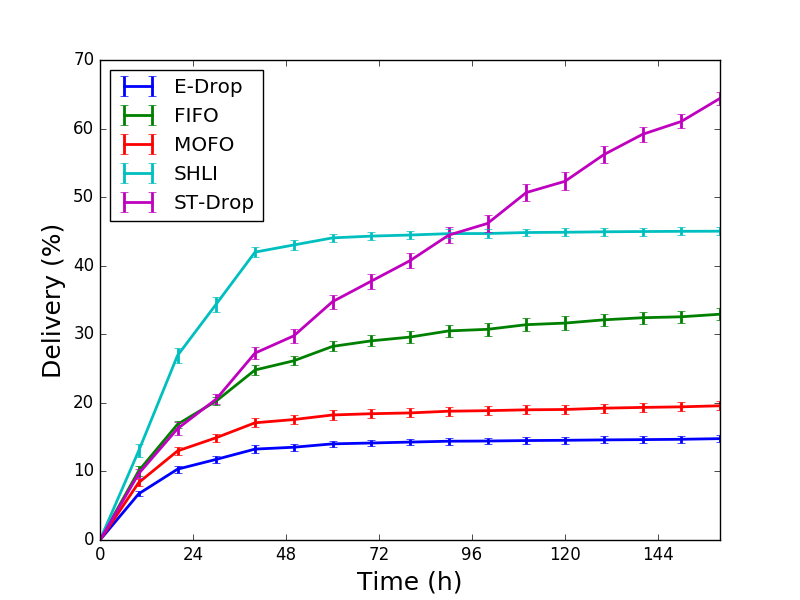
\includegraphics[width=\linewidth]{imgs/nccu/100/Epidemic-delivery.png}
        \caption{NCCU100 - Delivery Epidemic}
        \label{fig:nccu100EpidemicDel}
    \end{subfigure}
    \hfill %%
    \begin{subfigure}[b]{0.5\columnwidth}
        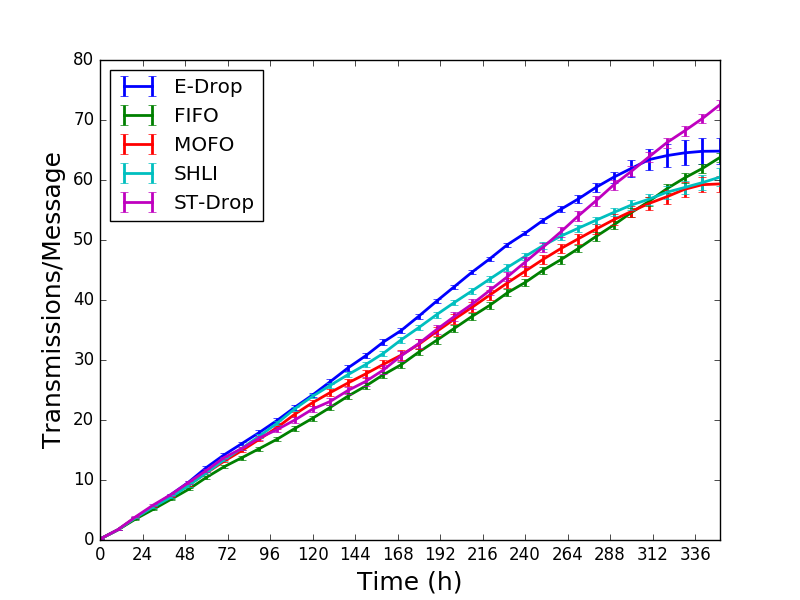
\includegraphics[width=\linewidth]{imgs/nccu/100/Epidemic-overhead.png}
        \caption{NCCU100 - Overhead Epidemic}
        \label{fig:nccu100EpidemicOver}
    \end{subfigure}

    \begin{subfigure}[b]{0.5\columnwidth}
        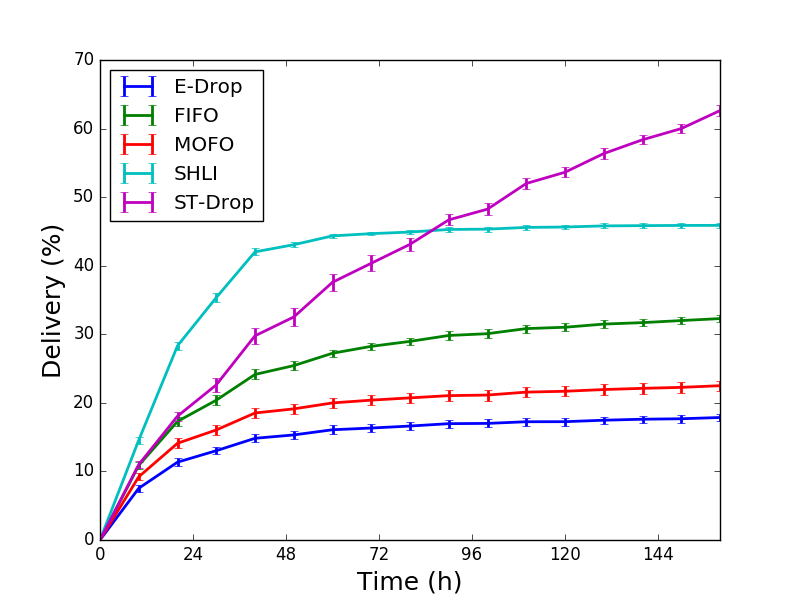
\includegraphics[width=\linewidth]{imgs/nccu/100/Prophet-delivery.png}
        \caption{NCCU100 - Delivery Prophet}
        \label{fig:nccu100ProphetDel}
    \end{subfigure}
    \begin{subfigure}[b]{0.5\columnwidth}
        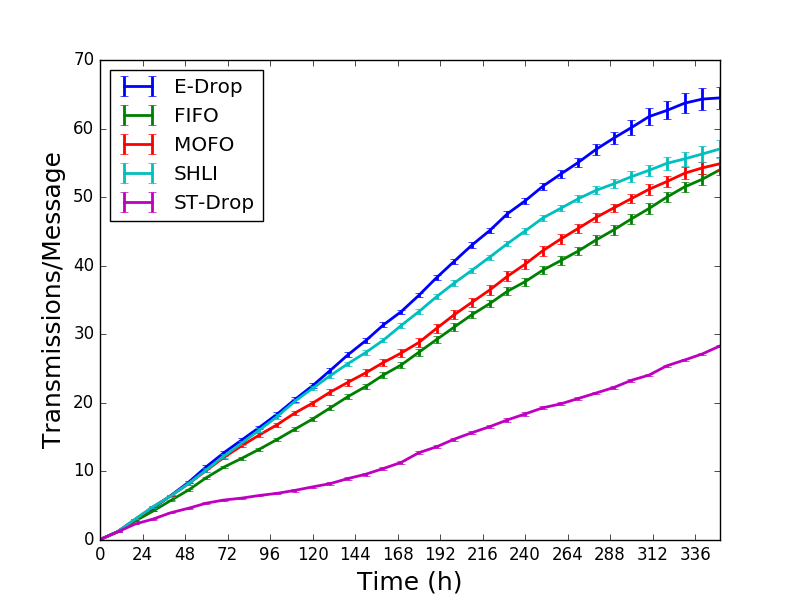
\includegraphics[width=\linewidth]{imgs/nccu/100/Prophet-overhead.png}
        \caption{NCCU100 - Overhead Prophet}
        \label{fig:nccu100ProphetOver}
    \end{subfigure}

    \begin{subfigure}[b]{0.5\columnwidth}
        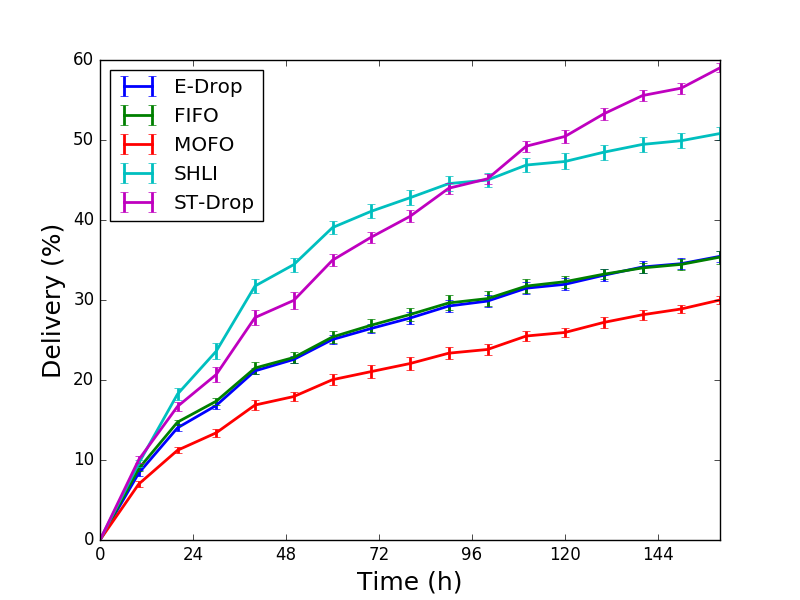
\includegraphics[width=\linewidth]{imgs/nccu/100/BubbleRap-delivery.png}
        \caption{NCCU100 - Delivery Bubble}
        \label{fig:nccu100BubbleDel}
    \end{subfigure}
    \begin{subfigure}[b]{0.5\columnwidth}
        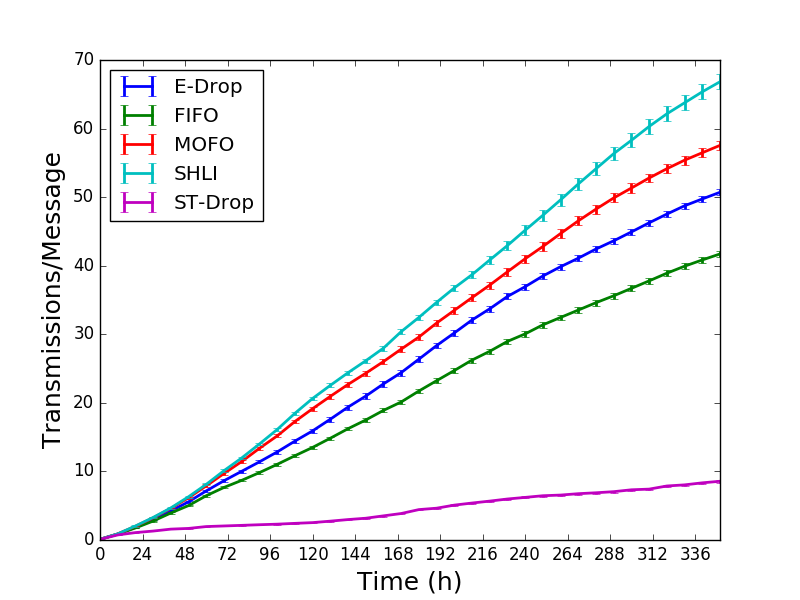
\includegraphics[width=\linewidth]{imgs/nccu/100/BubbleRap-overhead.png}
        \caption{NCCU100 - Overhead Bubble}
        \label{fig:nccu100BubbleOver}
    \end{subfigure}

    \caption{Comparison of message drop policies in the NCCU trace with 100\% traffic}
    \label{fig:nccu100}
\end{figure}

% images nccu 50
\begin{figure}
    \begin{subfigure}[b]{0.5\columnwidth}
        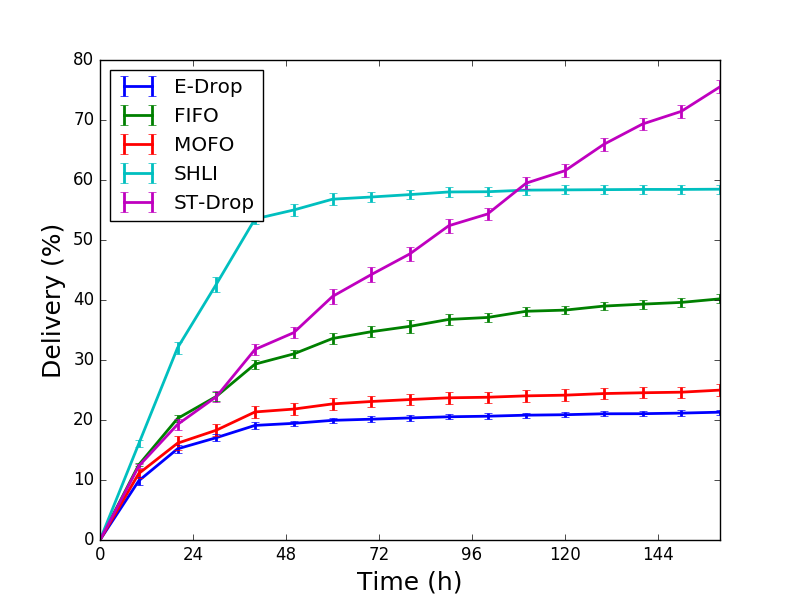
\includegraphics[width=\linewidth]{imgs/nccu/50/Epidemic-delivery.png}
        \caption{NCCU50 - Delivery Epidemic}
        \label{fig:nccu50EpidemicDel}
    \end{subfigure}
    \hfill %%
    \begin{subfigure}[b]{0.5\columnwidth}
        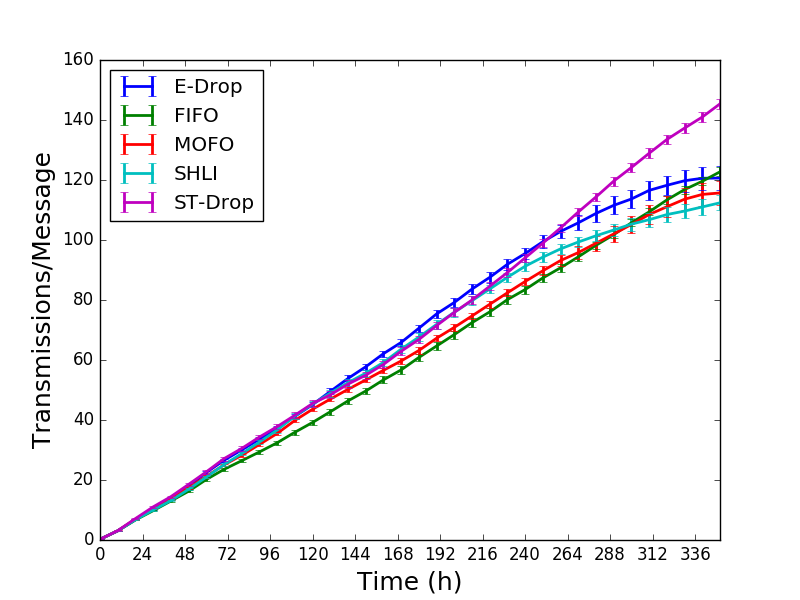
\includegraphics[width=\linewidth]{imgs/nccu/50/Epidemic-overhead.png}
        \caption{NCCU50 - Overhead Epidemic}
        \label{fig:nccu50EpidemicOver}
    \end{subfigure}

    \begin{subfigure}[b]{0.5\columnwidth}
        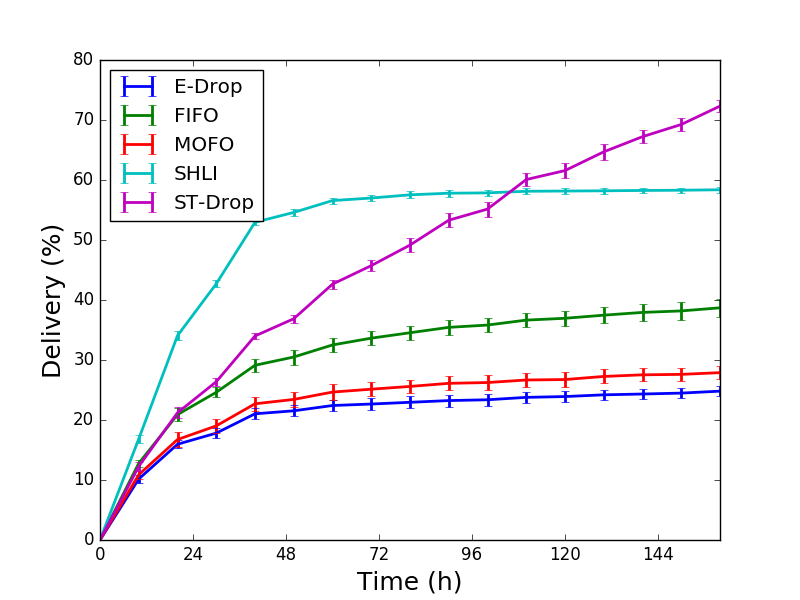
\includegraphics[width=\linewidth]{imgs/nccu/50/Prophet-delivery.png}
        \caption{NCCU50 - Delivery Prophet}
        \label{fig:nccu50ProphetDel}
    \end{subfigure}
    \begin{subfigure}[b]{0.5\columnwidth}
        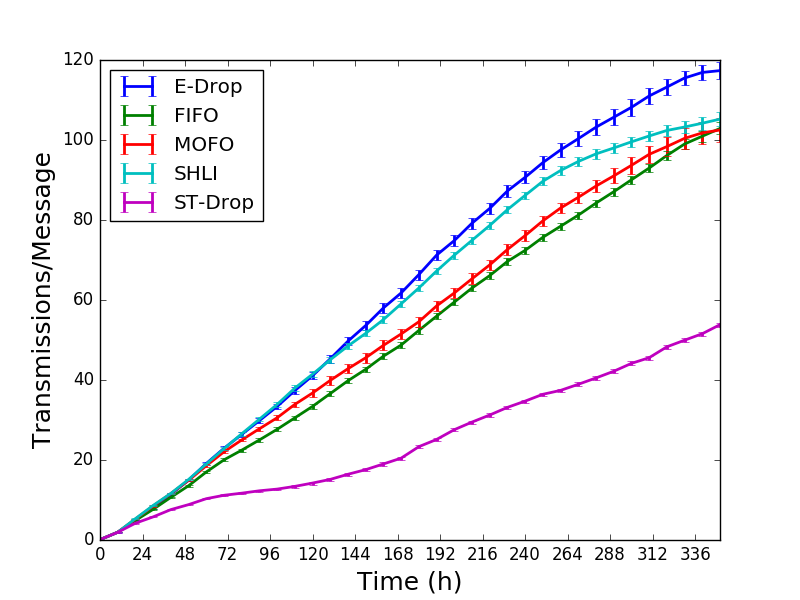
\includegraphics[width=\linewidth]{imgs/nccu/50/Prophet-overhead.png}
        \caption{NCCU50 - Overhead Prophet}
        \label{fig:nccu50ProphetOver}
    \end{subfigure}

    \begin{subfigure}[b]{0.5\columnwidth}
        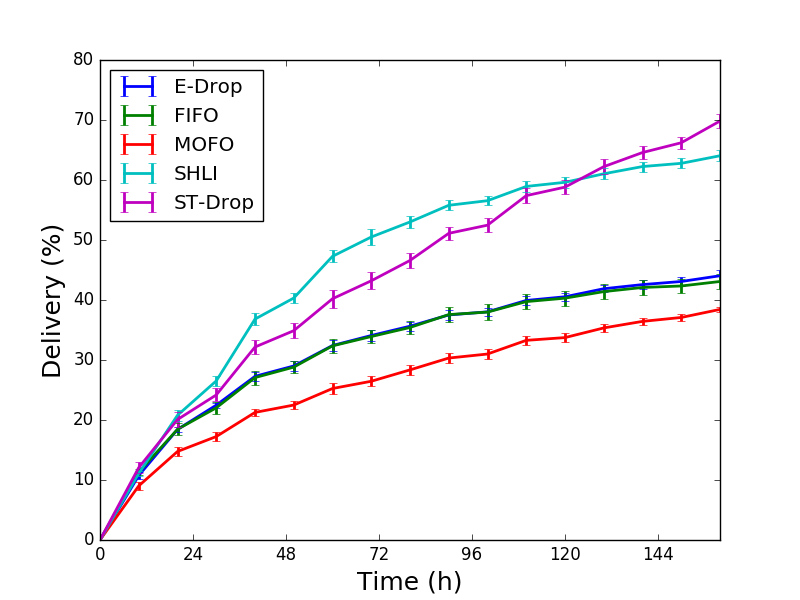
\includegraphics[width=\linewidth]{imgs/nccu/50/BubbleRap-delivery.png}
        \caption{NCCU50 - Delivery Bubble}
        \label{fig:nccu50BubbleDel}
    \end{subfigure}
    \begin{subfigure}[b]{0.5\columnwidth}
        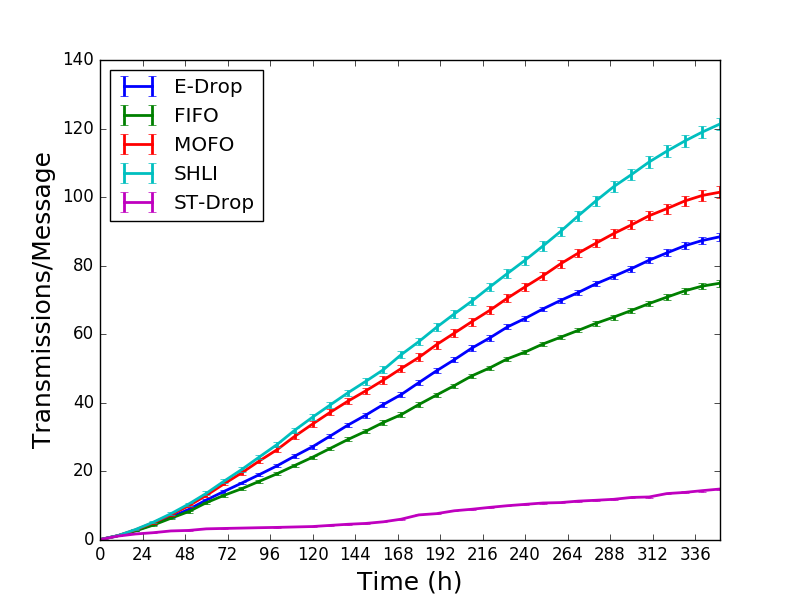
\includegraphics[width=\linewidth]{imgs/nccu/50/BubbleRap-overhead.png}
        \caption{NCCU50 - Overhead Bubble}
        \label{fig:nccu50BubbleOver}
    \end{subfigure}

    \caption{Comparison of message drop policies in the NCCU trace with 50\% traffic}
    \label{fig:nccu50}
\end{figure}

% images swim 100
\begin{figure}
    \begin{subfigure}[b]{0.5\columnwidth}
        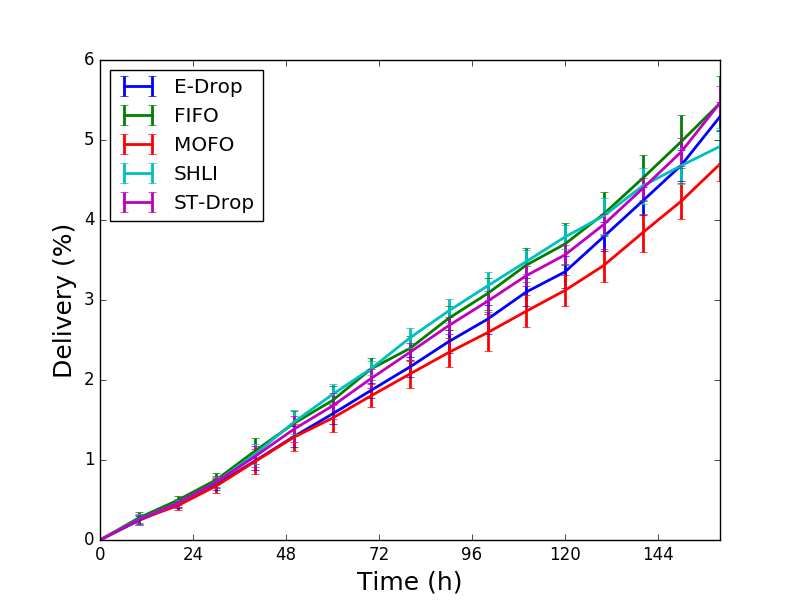
\includegraphics[width=\linewidth]{imgs/swim/100/Epidemic-delivery.png}
        \caption{SWIM100 - Delivery Epidemic}
        \label{fig:swim100EpidemicDel}
    \end{subfigure}
    \hfill %%
    \begin{subfigure}[b]{0.5\columnwidth}
        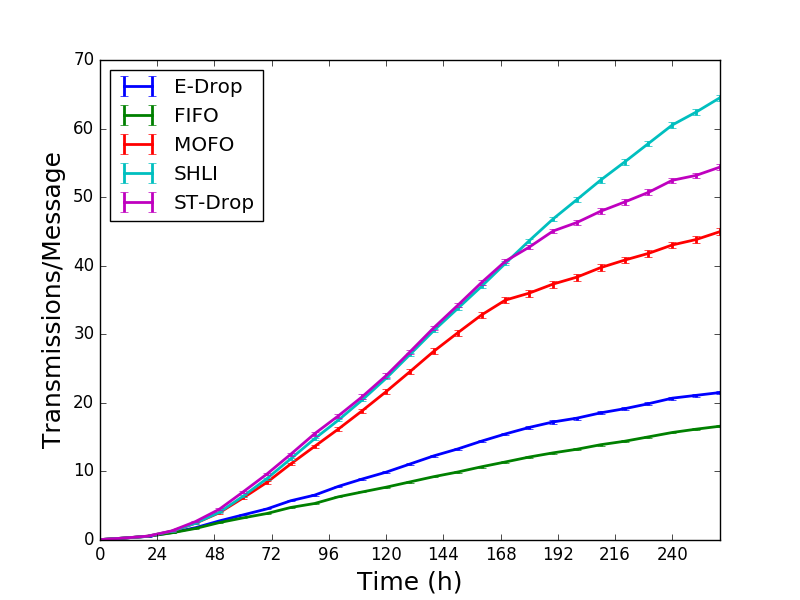
\includegraphics[width=\linewidth]{imgs/swim/100/Epidemic-overhead.png}
        \caption{SWIM100 - Overhead Epidemic}
        \label{fig:swim100EpidemicOver}
    \end{subfigure}

    \begin{subfigure}[b]{0.5\columnwidth}
        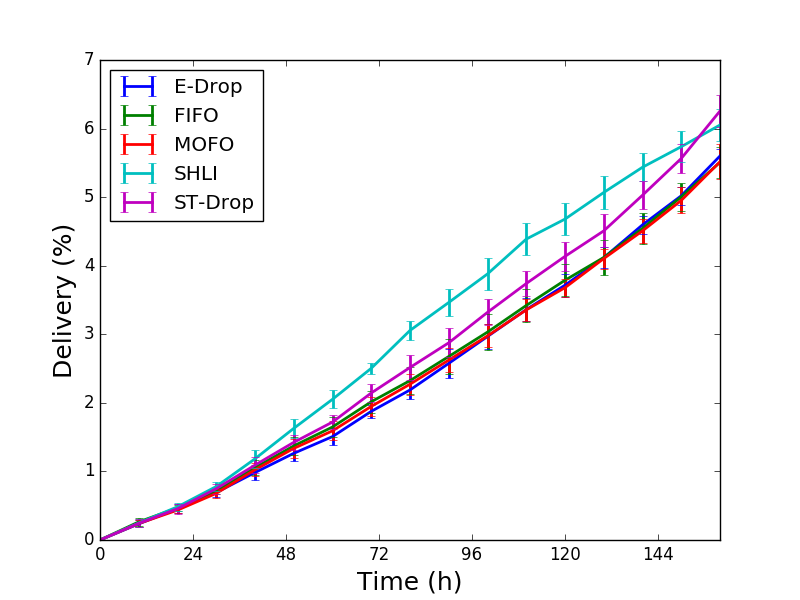
\includegraphics[width=\linewidth]{imgs/swim/100/Prophet-delivery.png}
        \caption{SWIM100 - Delivery Prophet}
        \label{fig:swim100ProphetDel}
    \end{subfigure}
    \begin{subfigure}[b]{0.5\columnwidth}
        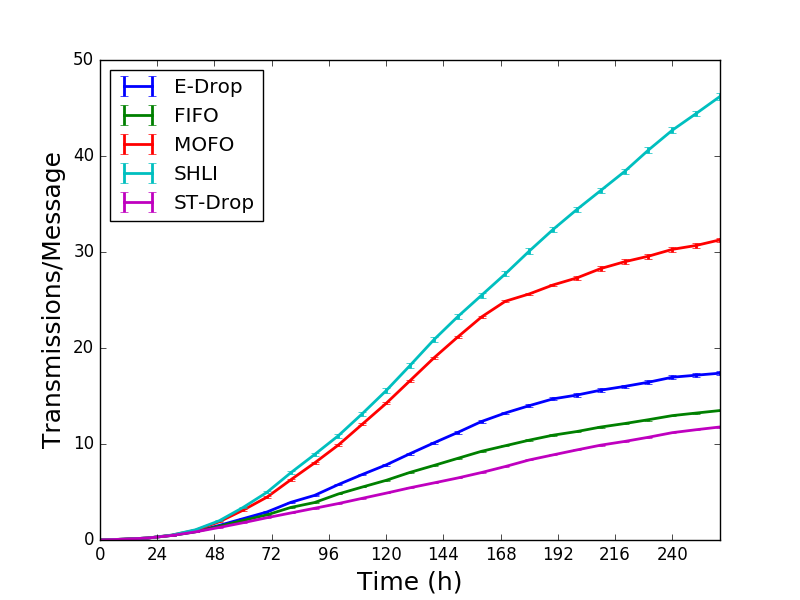
\includegraphics[width=\linewidth]{imgs/swim/100/Prophet-overhead.png}
        \caption{SWIM100 - Overhead Prophet}
        \label{fig:swim100ProphetOver}
    \end{subfigure}

    \begin{subfigure}[b]{0.5\columnwidth}
        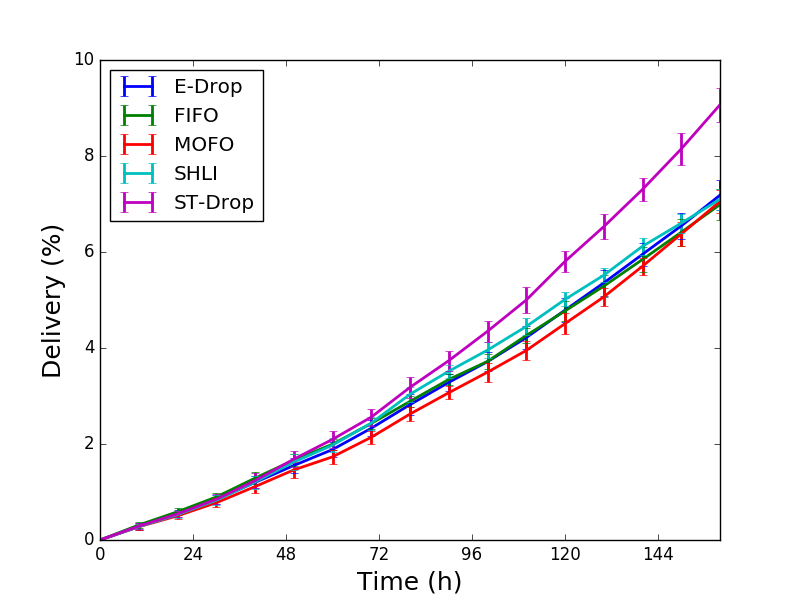
\includegraphics[width=\linewidth]{imgs/swim/100/BubbleRap-delivery.png}
        \caption{SWIM100 - Delivery Bubble}
        \label{fig:swim100BubbleDel}
    \end{subfigure}
    \begin{subfigure}[b]{0.5\columnwidth}
        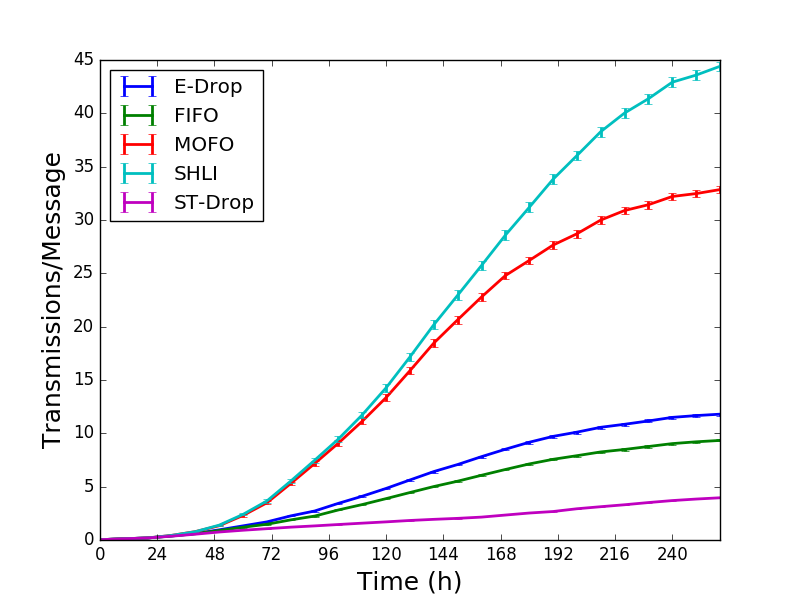
\includegraphics[width=\linewidth]{imgs/swim/100/BubbleRap-overhead.png}
        \caption{SWIM100 - Overhead Bubble}
        \label{fig:swim100BubbleOver}
    \end{subfigure}

    \caption{Comparison of message drop policies in the SWIM trace with 100\% traffic}
    \label{fig:swim100}
\end{figure}

% images swim 50
\begin{figure}
    \begin{subfigure}[b]{0.5\columnwidth}
        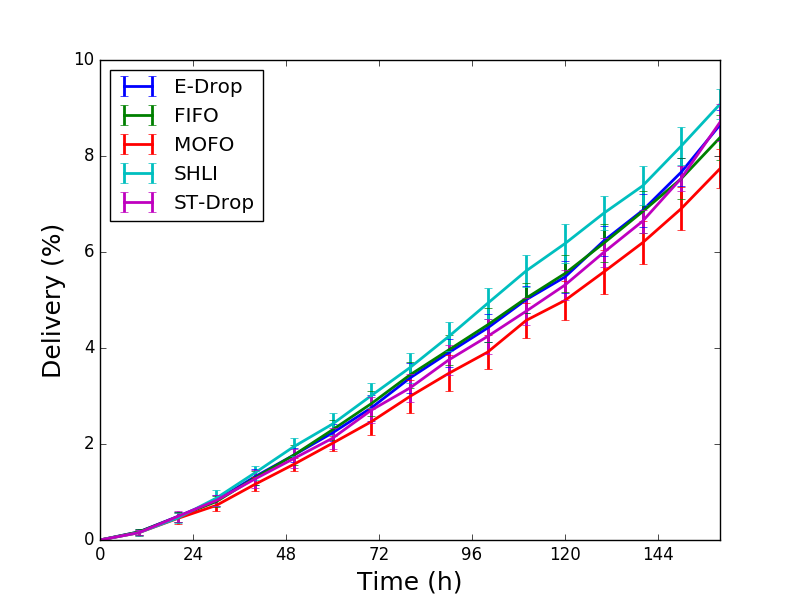
\includegraphics[width=\linewidth]{imgs/swim/50/Epidemic-delivery.png}
        \caption{SWIM50 - Delivery Epidemic}
        \label{fig:swim50EpidemicDel}
    \end{subfigure}
    \hfill %%
    \begin{subfigure}[b]{0.5\columnwidth}
        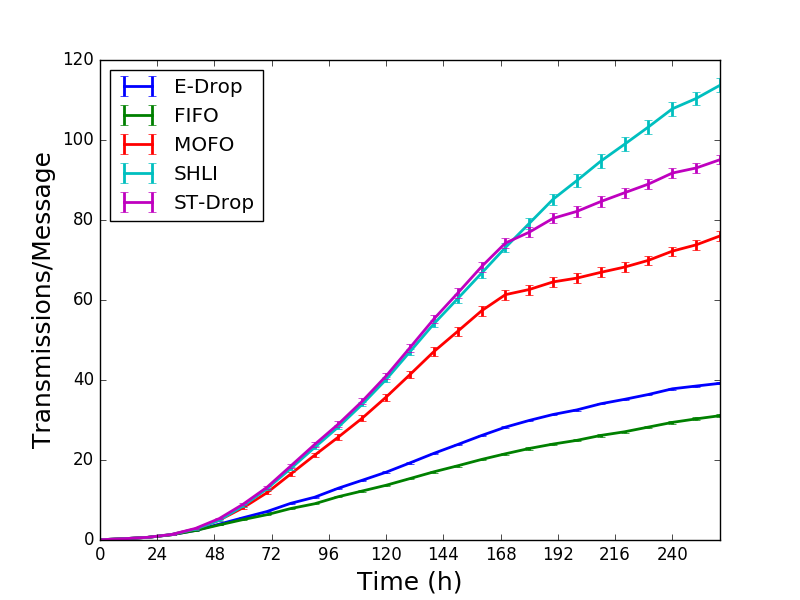
\includegraphics[width=\linewidth]{imgs/swim/50/Epidemic-overhead.png}
        \caption{SWIM50 - Overhead Epidemic}
        \label{fig:swim50EpidemicOver}
    \end{subfigure}

    \begin{subfigure}[b]{0.5\columnwidth}
        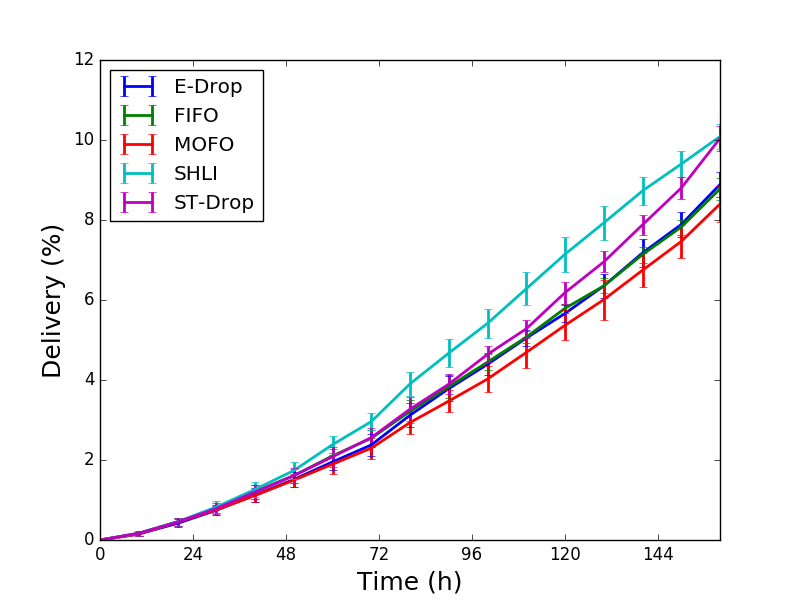
\includegraphics[width=\linewidth]{imgs/swim/50/Prophet-delivery.png}
        \caption{SWIM50 - Delivery Prophet}
        \label{fig:swim50ProphetDel}
    \end{subfigure}
    \begin{subfigure}[b]{0.5\columnwidth}
        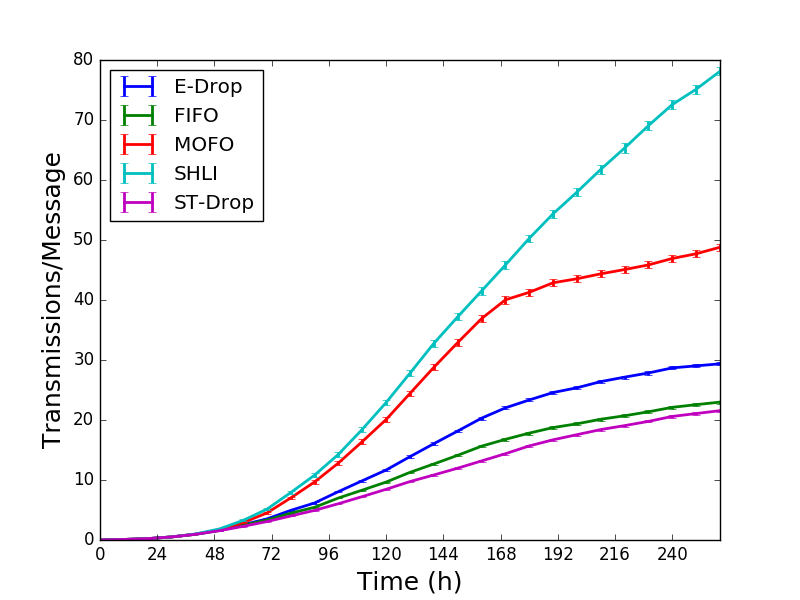
\includegraphics[width=\linewidth]{imgs/swim/50/Prophet-overhead.png}
        \caption{SWIM50 - Overhead Prophet}
        \label{fig:swim50ProphetOver}
    \end{subfigure}

    \begin{subfigure}[b]{0.5\columnwidth}
        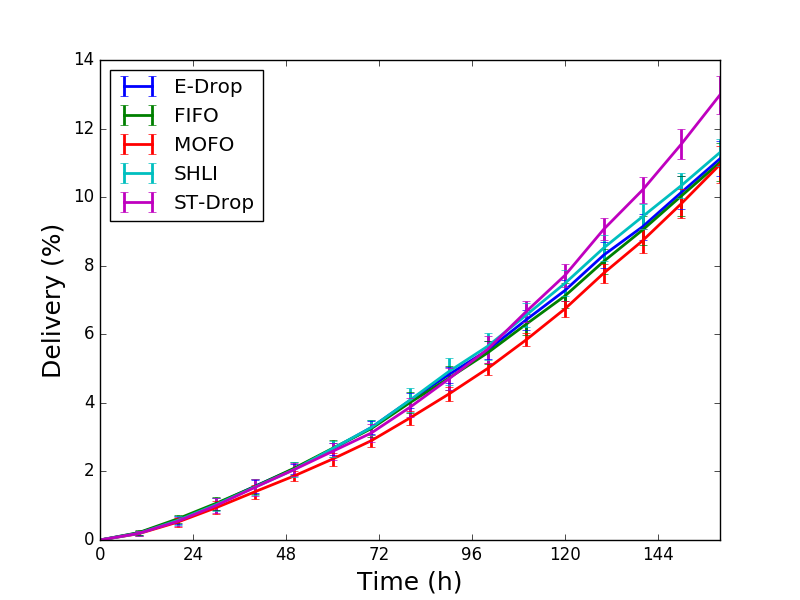
\includegraphics[width=\linewidth]{imgs/swim/50/BubbleRap-delivery.png}
        \caption{SWIM50 - Delivery Bubble}
        \label{fig:swim50BubbleDel}
    \end{subfigure}
    \begin{subfigure}[b]{0.5\columnwidth}
        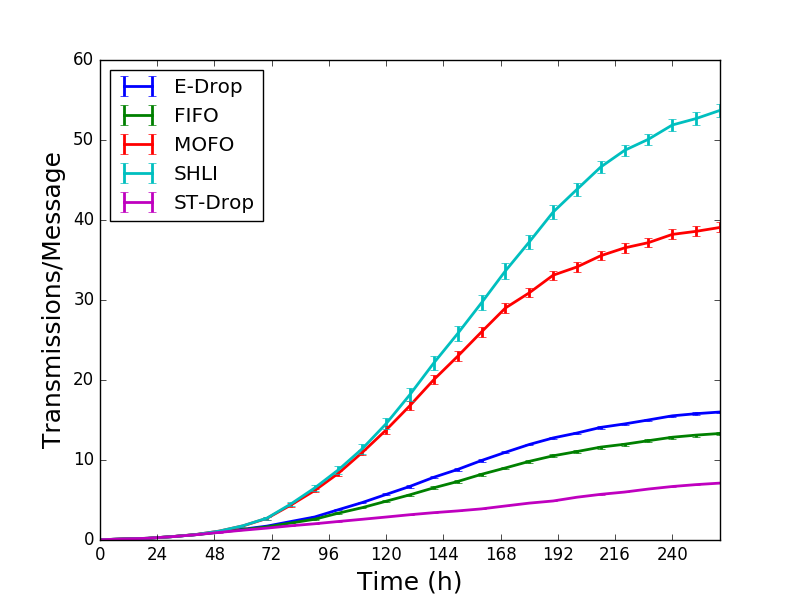
\includegraphics[width=\linewidth]{imgs/swim/50/BubbleRap-overhead.png}
        \caption{SWIM50 - Overhead Bubble}
        \label{fig:swim50BubbleOver}
    \end{subfigure}

    \caption{Comparison of message drop policies in the SWIM trace with 50\% traffic}
    \label{fig:swim50}
\end{figure}

The simulation results for NCCU100 and NCCU50 are presented in Figures \ref{fig:nccu100} and \ref{fig:nccu50}, respectively. The results of SWIM100 e SWIM50 are expressed in Figures \ref{fig:swim100} and \ref{fig:swim50}, respectively. The delivery ratio values were obtained considering the time spent to delivery each message since its creation time. The result is presented in a way that it can be analysed with different TTL values, for example, considering only points under the time value 48 in the x axis, we will get the delivery ratio with TTL of 48 hours.

Considering the Epidemic routing, the delivery ratio in the NCCU100 and NCCU50 scenarios is expressed in Figures \ref{fig:nccu100EpidemicDel} and \ref{fig:nccu50EpidemicDel}, respectively. We can see that the delivery ratio of ST-Drop policy is higher than E-Drop and MOFO for almost all the simulation time. It is also higher than FIFO for time values
higher than 48 hours and is higher than SHLI for time values higher than 120 hours. We can also see that the different traffic loads have not changed the behavior of the policies. The delivery ratio changed proportionally for the tested policies. The overhead results of NCCU100 and NCCU50 are expressed in Figures \ref{fig:nccu100EpidemicOver} and
\ref{fig:nccu50EpidemicOver}, respectively. In these two figures, we can see that the overhead results in the two traffic levels have similar behavior. All drop policies have overhead values very similar for almost all the simulation time. But we can see that in the last four days, ST-Drop continues to grow while others get small values. This is happening because in the last four days the delivery probability of ST-Drop continues to grow too, while other policies do not, consequently the overhead increase is
expected in Epidemic when more messages are delivered. The delivery ratios in the SWIM100 and SWIM50 scenarios are expressed in Figures \ref{fig:swim100EpidemicDel} and \ref{fig:swim50EpidemicDel}, respectively. In these figures, we can see that all drop policies have similar results for delivery ratio considering the confidence interval.
And, as in NCCU scenario, with both traffic levels, we can see a similar behavior. The overhead in the SWIM100 and SWIM50 scenarios is expressed in Figures \ref{fig:swim100EpidemicOver} and \ref{fig:swim50EpidemicOver}, respectively. Again, we can see similar behavior under the two traffic levels.

Considering the Prophet algorithm, the delivery ratio in the NCCU100 and NCCU50 scenarios is expressed in Figures \ref{fig:nccu100ProphetDel} and \ref{fig:nccu50ProphetDel}, respectively. We can see that the delivery ratio of ST-Drop is higher than FIFO, MOFO and E-Drop for almost all time values, and is higher than SHLI for time values higher than 120 hours. Again, we can see that under different traffic levels the results show similar behavior. The overhead in the NCCU100 and NCCU50 scenarios is expressed in Figures \ref{fig:nccu100ProphetOver} and \ref{fig:nccu50ProphetOver}, respectively. We can see again that the results show similar behavior for both traffic levels. In this case, ST-Drop obtained the best results during all simulation time. The delivery ratio in the SWIM100 and SWIM50 scenarios is expressed in Figures \ref{fig:swim100ProphetDel} and \ref{fig:swim50ProphetDel}, respectively. Again, we see similar behavior under both traffic levels. The delivery ratio is similar for all drop policies, except for time values between 72 and 144 hours where SHLI obtained slightly better results. The overhead in the SWIM100 and SWIM50 is expressed in Figures \ref{fig:swim100ProphetOver} and \ref{fig:swim50ProphetOver}, respectively. In this case, we obtained the same behavior of NCCU scenarios, in which ST-Drop obtained the best results during all simulation time.

Finally, we analyze the policies when used with Bubble Rap routing. The delivery ratio in the NCCU100 and NCCU50 scenarios is expressed in Figures \ref{fig:nccu100BubbleDel} and \ref{fig:nccu50BubbleDel}, respectively. We can see similar behavior under both traffic levels. The ST-Drop obtained a higher delivery ratio than FIFO, E-DROP and MOFO for almost all time values, and higher values than SHLI for time values higher than 120. The overhead in the NCCU100 and NCCU50 scenarios is expressed in Figures \ref{fig:nccu100BubbleOver} and \ref{fig:nccu50BubbleOver}, respectively. As with Prophet routing, in this scenario the ST-Drop obtained the best results during all simulation time, and we can see similar behavior under both traffic levels. The delivery ratio in the SWIM100 and SWIM50 scenarios is expressed in Figures \ref{fig:swim100BubbleDel} and \ref{fig:swim50BubbleDel}, respectively. Again, we see similar behavior under both traffic levels. The delivery ratio is similar for all drop policies, but ST-Drop obtained slightly better results for time values greater than 120 hours. The overhead in the SWIM100 and SWIM50 is expressed in Figures \ref{fig:swim100BubbleOver} and \ref{fig:swim50BubbleOver}, respectively. In this case, we obtained the same behavior of NCCU scenarios, in which ST-Drop obtained the best
results during all simulation time.

In general, the ST-Drop policy obtained better delivery ratio values for all the three routing algorithms. For the overhead ratio, ST-Drop obtained the best results in all scenarios with Prophet and Bubble Rap routing algorithms. The SHLI policy obtained better results with low TTLs because in this policy, messages that spent more time in the network are dropped first, so it is expected that most delivered messages, when using this policy, have low delivery time. But when we consider all TTL range, ST-Drop obtained better results than SHLI.

It is worth mentioning that, in the Prophet algorithm, the ST-Drop overhead was much lower when compared to the other strategies. With respect to Bubble Rap, this result is even better, since ST-Drop reaches overhead values that are three times smaller than the second-best policy. This latter observation is particularly important because, as of today, social-aware algorithms such as Bubble Rap are considered the state-of-art for cost-effective opportunistic routing. This assertion can be reassured by contrasting the delivery ratio and overhead values for Epidemic, Prophet, and Bubble Rap. In both mobility traces, we can see that Bubble Rap achieves the best delivery ratio and the lowest overhead, especially when used together with ST-Drop.
\chapter{Conclusion}
\label{ch:Conclusion}
Put some text here

% Bibliografia
\ppgccbibliography{bibliography}

\end{document}